% EMBER — BIP 2026
%
% Every measured number goes through \result{key}{value}: the macro prints the
% value and `ember.paper_sync.verify_paper` checks that it matches results/. A
% number written by hand is a number nobody is verifying.
%
%   uv run python -c "from ember.paper_sync import render_tables; render_tables()"
%   uv run python -c "from ember.paper_sync import verify_paper; print(verify_paper('paper/main.tex'))"

\documentclass[conference]{IEEEtran}
\usepackage{amsmath,amssymb}
\usepackage{booktabs}
\usepackage{graphicx}
\usepackage[hidelinks]{hyperref}

% Generado por ember.paper_sync. No editar a mano.
%
% \result{clave}{valor} imprime el valor y deja registrada su procedencia.
% `ember.paper_sync.verify_paper` verifica que el valor coincida con lo medido
% en results/. Un número sin macro es un número que nadie está verificando.
\newcommand{\result}[2]{#2}


\title{Two regimes of bioinspired memory:\\an architecture-search perspective}
\author{\IEEEauthorblockN{Anonymous --- double-blind review}}

\begin{document}
\maketitle

\begin{abstract}
We present EMBER, a research program on long-term episodic memory for cognitive
robots, with four empirical contributions. First, an exhaustive search over a
discrete space of
\result{exp03_axis_liveness:n_genotipos|int}{576} bioinspired mechanisms
---derived from Sparse Distributed Memory, engram consolidation and trace
decay--- reveals a threshold law: when the ratio between recurring experience
prototypes and memory capacity ($r = K_{proto}/C$) drops below 1, merge
consolidation explains
\result{exp02_threshold_grid:regimenes.compression.eta2_write|pct}{73.0}\,\%
of performance variance; above the threshold that figure falls to
\result{exp02_threshold_grid:regimenes.selection.eta2_write|pct}{1.6}\,\%
and minimum-strength forgetting dominates. Second, a two-phase benchmark
evaluates four architectures, separating reconstruction fidelity from retention
under capacity pressure: SDM with a prediction-error gate achieves perfect
rare-event retention
(\result{exp04_arch_benchmark:architectures.SDM.battery.per_task.rare_retention}{1.000})
against
\result{exp04_arch_benchmark:architectures.FIFO.battery.per_task.rare_retention}{0.038}
for the FIFO buffer of the deployed e-MDB architecture. Third, instrumenting the
same law on real perceptual embeddings (CIFAR-100, ResNet-18) exposes a
precondition the synthetic design does not reveal: if the domain's
intra-prototype similarity does not reach the consolidation threshold ---here,
\result{exp05_real_embeddings:precondicion_cifar100.similitud_intra_prototipo|f3}{0.401}
against a threshold of
\result{exp05_real_embeddings:precondicion_cifar100.umbral_de_fusion|f2}{0.85}---,
the write axis becomes inoperative and there is no compression regime for any
$r$; the variance explained by writing falls between
\result{exp05_real_embeddings:dominios.cifar100.celdas.4.eta2_write|pct}{0.0}\,\%
and
\result{exp05_real_embeddings:dominios.cifar100.celdas.1.eta2_write|pct}{0.4}\,\%
across the five cells of the sweep. Fourth, we validate the salience mechanism
in MiniGrid under partial observability: with a perceptual surprise signal,
rare-event retention stays at the floor, but anchoring it in reward-prediction
error ---without changing genotype or policy--- raises it from
\result{exp06_minigrid:comparacion_aleatoria_prediccion.resultados.frontera.tasa|pct}{0.0}\,\%
to
\result{exp06_minigrid:comparacion_aleatoria_recompensa.resultados.frontera.tasa|pct}{52.6}\,\%,
while the FIFO, which does not read that signal, does not move.
\end{abstract}

\begin{IEEEkeywords}
bioinspired memory, neural architecture search, Sparse Distributed Memory,
engram consolidation, episodic memory, lifelong learning
\end{IEEEkeywords}

% ═══════════════════════════════════════════════════════════════════════
\section{Introduction}

A cognitive robot that learns over its lifetime faces a memory problem that goes
well beyond mere storage. It must decide what is worth keeping, keep that
information accessible in proportion to its relevance, and retrieve it reliably
even from a partial or degraded cue. These three requirements map onto three
well-studied properties of biological memory: selective encoding modulated by
surprise and novelty, use-regulated trace consolidation and decay, and
content-addressable retrieval that is robust to noise.

The episodic buffer of the e-MDB architecture \cite{emdb2021} ---a
fixed-capacity FIFO queue--- satisfies none of the three. It keeps whatever was
perceived most recently, treating every experience alike regardless of its
importance, novelty or prediction error. Retrieval is sequential, not by
content. When the buffer fills, the oldest episode is simply discarded: it is,
in effect, a database with no criterion.

The bioinspired-memory literature offers several principled remedies. Kanerva's
Sparse Distributed Memory (SDM) \cite{kanerva1988} provides content-addressable
retrieval over a distributed superposition of memory locations, with graceful
degradation under noise. Hebbian engram consolidation \cite{liu2012,hebb1949}
offers a biologically plausible mechanism for reinforcing traces through
repeated co-activation. Prediction-error gating \cite{cole2015}, grounded in the
neurobiological role of dopamine, regulates how strongly a new experience is
encoded as a function of how surprising it is. And selective-forgetting policies
based on trace strength or utility \cite{murdock1962} give a criterion for what
to discard when capacity is exceeded.

But these mechanisms are almost always evaluated in isolation, embedded in
architectures purpose-built to show them off, and compared against baselines
that do not share their design space. That makes it hard ---sometimes
impossible--- to tell whether a reported gain comes from the mechanism itself or
from an incidental advantage of the evaluation protocol.

This work inverts the usual approach. Rather than proposing a new architecture
and arguing that it beats a simple baseline, we define a discrete design space
in which each bioinspired mechanism is an axis, and we traverse it
exhaustively. The e-MDB FIFO is not treated as a baseline external to the
comparison: it is one more point inside the same search space. This choice
turns a potentially circular comparison into a falsifiable question ---given the
full space, where does the deployed incumbent land, and which combination of
mechanisms defines the performance frontier?

We then evaluate the individual bioinspired architectures that emerge from that
analysis with a two-phase benchmark that explicitly separates the ability to
reconstruct a degraded cue (a prerequisite of any useful associative memory)
from the harder problem of retaining the right episodes under continuous
capacity pressure (the realistic condition of a robot operating across its
entire service life). Finally, we instrument the threshold law and the salience
mechanism on two real domains ---perceptual embeddings and a navigation
environment under partial observability--- to expose preconditions that no
synthetic design reveals on its own, and we show that at least one of them is
corrected by identifying which signal should feed the strength gate.

The main contributions of this work are:

\begin{itemize}
  \item A \emph{threshold law}: the ratio $r = K_{proto}/C$ determines which
  family of mechanisms governs performance, with a regime transition that
  reproduces independently across three distinct capacities ---and, within the
  selection regime that this law defines, modulating encoding strength by
  novelty and prediction error, the most-cited mechanism in the
  bioinspired-memory literature, explains barely
  \result{exp01_nas_full:main_effects.3.eta2|pct}{1.4}\,\% of the variance as a
  main effect yet produces a
  \result{exp01_nas_full:salience_conditional_ratio|f2}{14.41}$\times$
  improvement in rare-event retention when combined with minimum-strength
  eviction.
  \item A two-phase benchmark that admits architectures by reconstruction
  before exposing them to capacity pressure, revealing that a pure spiking
  circuit (LIF + STDP) does not transfer to the continuous-vector domain
  without an intermediate encoding layer.
  \item A precondition for the threshold law ---the reachability of the merge
  threshold--- which on CIFAR-100 turns out to be the dominant variable: there
  is no $r$, nominal or effective, at which a compression regime exists.
  \item An analogous precondition for the salience mechanism, identified and
  corrected on a real environment under partial observability: surprise must be
  anchored in the variable that decides what matters (reward), not in the
  perceptual novelty of the state.
\end{itemize}

% ═══════════════════════════════════════════════════════════════════════
\section{Related work}

\subsection{Sparse Distributed Memory}

Kanerva's Sparse Distributed Memory \cite{kanerva1988} is a computational model
of associative memory inspired by the high-dimensional structure of the nervous
system. Its central idea is that storing information in a single location is
fragile; instead, patterns should be distributed across many overlapping
locations, so that a noisy or partial query still activates enough of those
same locations to reconstruct the original. An SDM consists of fixed
\emph{hard locations} with random addresses; a write activates the locations
within a similarity radius of the queried address, and a read sums and
thresholds those same locations. The key property is graceful degradation:
nearby addresses activate partially overlapping sets, so a corrupted query
still recovers the stored pattern as long as the memory is not overloaded. In
EMBER's adaptation, the address space is replaced by continuous unit vectors,
and activation is by inner product rather than Hamming radius; \cite{kanerva2009}
extends the same intuition to hyperdimensional computing.

\subsection{Engrams and Hebbian consolidation}

The concept of the engram ---the physical trace a memory leaves in neural
tissue--- was coined by Semon \cite{semon1904} and confirmed experimentally in
modern neuroscience: specific neuronal populations activate during learning and
reactivate during recall \cite{liu2012}. The cellular mechanism underlying
engram formation is long-term potentiation (LTP): when two neurons fire
together repeatedly, the synapse connecting them strengthens. This is the
principle Hebb \cite{hebb1949} distilled into his dictum: cells that fire
together wire together. In EMBER's ENN instantiation this becomes a matrix of
fast Hebbian weights, updated online without backpropagation: each write
creates a new trace or reinforces an existing one if it exceeds the
cosine-similarity threshold, with an initial strength proportional to the
prediction error of the incoming experience and exponential decay in the
absence of reinforcement.

\subsection{Spike-timing-dependent plasticity}

Biological neurons communicate through discrete electrical pulses. The relative
timing between those pulses carries information that a rate-based neuron
discards. Spike-timing-dependent plasticity (STDP) \cite{bipoo1998} is a
Hebbian rule at the level of the individual spike: a synapse strengthens if the
presynaptic neuron fires just before the postsynaptic one, and weakens in the
opposite order. This rule groups neurons into assemblies: when a group
co-activates repeatedly, STDP strengthens the group's internal connections more
than its external ones, leaving a structural trace that is, precisely, an
engram. In EMBER's PoC-3 we verified this on a network of leaky
integrate-and-fire (LIF) neurons organized into groups: after repeated
presentations via forced bursts, intra-group weights rose well above
inter-group weights, and a partial cue from one group was enough to recruit the
rest of its neurons without activating the other groups. In this work we test
whether that same mechanism ---which operates natively on discrete neural
activation patterns--- extends to continuous input vectors.

\subsection{Architecture search for memory modules}

Neural architecture search (NAS) \cite{elsken2019} automates the design of
neural-network components by treating architectural decisions as optimizable
variables. Its application to the design of the memory mechanism itself ---
rather than its integration with a downstream task--- is far less explored. The
closest prior work, Neural Turing Machines \cite{graves2014} and related
differentiable-memory architectures (e.g. \cite{munkhdalai2017}), fixes the
memory type (externally addressable) and searches over the read/write heads and
attention mechanisms. Our contribution is to make the fundamental memory
mechanism the search variable, and to use a fully enumerable discrete space so
that no result can be attributed to the behavior of an approximate optimizer.

\subsection{Prioritized replay and episodic memory in reinforcement learning}

Outside neuroscience, the closest analogue to the strength-gate / content-read
pair this work studies comes from deep reinforcement learning. Prioritized
experience replay \cite{schaul2016} weights which transition to revisit by its
temporal-difference error ---the same ``surprising things count more''
principle that motivates prediction-error strength gating--- and Neural
Episodic Control \cite{pritzel2017} uses a differentiable dictionary indexed by
similarity, analogous to SDM's content-addressable read, to bootstrap action
values from stored episodes. In both cases the priority or read mechanism is a
design component chosen in advance and evaluated in isolation. This work treats
that choice itself ---which signal to prioritize, which read policy, which
eviction policy--- as the search space, and measures in which regime each one
matters and in which it does not.

\subsection{The e-MDB architecture and the LOLA problem}

e-MDB (\emph{epistemic Multilevel Darwinist Brain}) \cite{emdb2021} is a
ROS2-based cognitive architecture designed to address the LOLA problem
(\emph{Lifelong Open-ended Learning Autonomy}): building a robot that acquires
and relates knowledge autonomously and continuously, with no predefined goals
or task boundaries. It organizes all its cognitive components as
\emph{Cognitive Nodes} with a common interface, and uses an \texttt{Episode}
object as the unit of experience. Its episodic-memory component,
\texttt{EpisodicBuffer}, is a fixed-size \texttt{deque}: new episodes are
appended and the oldest are discarded automatically when the limit is reached.
There is no importance criterion, no similarity-based retrieval, and no
consolidation mechanism. In the NAS formulation of Section \ref{sec:nas}, this
corresponds exactly to the genotype
\texttt{\{read: nn, write: append, strength: constant, decay: 1.0, evict: fifo,
reinforce: 0.0\}} ---one point among 576 in the design space.

% ═══════════════════════════════════════════════════════════════════════
\section{Search over a bioinspired design space}
\label{sec:nas}

\subsection{Design space and genotype encoding}

We encode each candidate memory architecture as a discrete six-axis genotype,
each axis motivated by a distinct biological or computational principle. Table
\ref{tab:axes} lists the axes, their options, and the corresponding biological
inspiration. The Cartesian product yields
\result{exp03_axis_liveness:n_genotipos|int}{576} candidate genotypes.

\begin{table}[t]
\centering
\caption{Bioinspired design space. The Cartesian product yields 576 candidate
genotypes, exhaustively enumerable.}
\label{tab:axes}
\begin{tabular}{p{1.5cm}p{2.6cm}p{3.3cm}}
\hline
Axis & Options & Biological root \\
\hline
\texttt{read} & nn / topk3 / radius & Episodic retrieval vs. activation circle
(Kanerva) \\
\texttt{write} & append / merge & Trace creation vs. Hebbian merge
consolidation \\
\texttt{strength} & constant / novelty / pred\_error / both & LTP gating by
salience and surprise (dopamine) \\
\texttt{decay} & 1.0 / 0.995 / 0.98 & Synaptic weakening without reinforcement \\
\texttt{evict} & fifo / min\_strength / min\_utility / random & Forgetting by age
vs. by importance \\
\texttt{reinforce} & 0 / 0.5 & LTP by reactivation \\
\hline
\end{tabular}
\end{table}

The \emph{read} axis operationalizes how past experiences are retrieved:
\texttt{nn} returns the single closest stored episode; \texttt{topk3}
aggregates the three closest; \texttt{radius} implements the full SDM read,
superposing all traces within a similarity radius relative to the best match.
The \emph{write} axis controls trace creation: \texttt{append} always creates a
new trace; \texttt{merge} first checks whether a sufficiently similar trace
already exists (cosine similarity $\geq 0.85$) and, if so, reinforces it
instead of creating a redundant copy ---the computational analogue of Hebbian
consolidation. The \emph{initial-strength} axis ---the \emph{strength gate},
which elsewhere in the text we also call the \emph{salience gate} when the
emphasis is on which biological signal opens it--- modulates how much weight a
new experience receives at encoding time: \texttt{constant} assigns a fixed
weight; the other three options introduce a biological signal ---novelty,
prediction error, or the two combined. The \emph{decay} axis determines whether
the strength of stored traces erodes over time without reinforcement. The
\emph{eviction} axis controls what is forgotten when memory fills:
\texttt{fifo} discards the oldest (the e-MDB default), \texttt{min\_strength}
discards the weakest trace, \texttt{min\_utility} discards the least-queried,
and \texttt{random} discards at random. The \emph{read-reinforcement} axis
models LTP by reactivation: each time an episode is retrieved, its strength
increases.

An early version of this space had two silently dead axes ---the pilot reported
576 genotypes but only 96 were functionally distinct, because \texttt{read} and
\texttt{reinforce} changed the outcome for no pair of sibling genotypes. Both
faults were repaired: \texttt{read} because its three modes now do different
things, and \texttt{reinforce} because the evaluation tasks interleave reads
between writes. \texttt{exp03\_axis\_liveness} verifies this property
automatically and runs in continuous integration so that no axis can die again
without the paper noticing.

\subsection{Axis observability}

A design axis that changes the outcome nowhere in the space is measuring
nothing, and any conclusion about the irrelevance of that mechanism is really a
conclusion about the instrument. Before reporting effects, we verify that all
six axes are observable: for each one we measure the maximum performance
difference between genotypes that differ only in that axis.

% Generado por ember.paper_sync. No editar a mano.
\begin{table}[t]
\centering
\caption{Efectos principales sobre el espacio completo. La columna de observabilidad es la máxima diferencia entre genotipos hermanos: un eje con $\eta^2$ nulo y observabilidad nula no está siendo medido.}
\label{tab:main-effects}
\begin{tabular}{lrrl}
\hline
Eje & $\eta^2$ & Observabilidad & Nota \\
\hline
write & 56.6\,\% & 0.583 &  \\
evict & 17.0\,\% & 0.728 &  \\
decay & 1.8\,\% & 0.645 &  \\
strength & 1.4\,\% & 0.711 &  \\
reinforce & 0.0\,\% & 0.206 &  \\
read & 0.0\,\% & 0.119 &  \\
\hline
\end{tabular}
\end{table}


Write mode is the strongest main effect
(\result{exp01_nas_full:main_effects.0.eta2|pct}{56.6}\,\%), followed by the
eviction policy (\result{exp01_nas_full:main_effects.1.eta2|pct}{17.0}\,\%).
Decay and initial strength explain much less as main effects
(\result{exp01_nas_full:main_effects.2.eta2|pct}{1.8}\,\% and
\result{exp01_nas_full:main_effects.3.eta2|pct}{1.4}\,\% respectively), and read
and read-reinforcement come out near zero
(\result{exp01_nas_full:main_effects.5.eta2|pct}{0.0}\,\% and
\result{exp01_nas_full:main_effects.4.eta2|pct}{0.0}\,\%). The difference from
the pilot is that both now have strictly positive observability
(\result{exp01_nas_full:main_effects.5.liveness|f3}{0.119} and
\result{exp01_nas_full:main_effects.4.liveness|f3}{0.206}): a null $\eta^2$ with
positive observability does not say the mechanism does not matter, it says its
effect is not a main effect ---Section \ref{sec:interaction} shows exactly that
case for initial strength.

The e-MDB FIFO ---genotype
\texttt{\{read: nn, write: append, strength: constant, decay: 1.0, evict: fifo,
reinforce: 0.0\}}--- scores
\result{exp01_nas_full:incumbent.score|f3}{0.106}, in the range
\result{exp01_nas_full:incumbent.rank_optimistic|int}{416}--%
\result{exp01_nas_full:incumbent.rank_pessimistic|int}{469} of 576, with
\result{exp01_nas_full:incumbent.n_tied|int}{54} ties. It is not the absolute
floor of the genotype space: below its pessimistic rank of
\result{exp01_nas_full:incumbent.rank_pessimistic|int}{469}\ there are
architectures that score strictly worse, almost all combining criterion-free
\texttt{append} writing with minimum-utility eviction or \texttt{topk3} reads
over compressed memory. The frontier of the space scores
\result{exp01_nas_full:frontier.score|f3}{0.818}: a factor of almost eight over
the incumbent.

\subsection{The regime transition}

The $56.6\,\%$ of write mode is not primarily a property of the merge
mechanism; it is a property of the relationship between the number of recurring
experience prototypes and memory capacity. We define the prototype-to-capacity
ratio $r = K_{proto}/C$ and sweep the effective architecture space over a grid
of capacities and ratios, controlling visits per prototype so that the ratio is
not confounded with stream recurrence.

% Generado por ember.paper_sync. No editar a mano.
\begin{table}[t]
\centering
\caption{Regime transition as a function of the prototype-to-capacity ratio $r = K_{proto}/C$.}
\label{tab:regimes}
\begin{tabular}{llrrr}
\hline
Regime & Range & Cells & $\eta^2$ write & $\eta^2$ evict \\
\hline
Compression & $r \leq  0.5$ & 9 & 73.0\,\% & 8.2\,\% \\
Transition & $0.5 < r < 1$ & 3 & 52.4\,\% & 10.6\,\% \\
Selection & $r \geq  1$ & 12 & 1.6\,\% & 16.3\,\% \\
\hline
\end{tabular}
\end{table}


The transition from ``consolidation dominates'' to ``eviction dominates'' falls
abruptly near $r=1$ across the three evaluated capacities (10, 20 and 40),
independently of $K_{proto}$: the estimated crossover (geometric mean over the
transition cell) is
\result{exp02_threshold_grid:r_umbral_medio|f2}{0.88}, with interval
[\result{exp02_threshold_grid:r_umbral_ci.0|f2}{0.87},
\result{exp02_threshold_grid:r_umbral_ci.1|f2}{0.89}]. Below $r=1$, merging
compresses the routine into fewer slots than it would otherwise occupy, and the
freed slots become available for the rare. Above $r=1$ there is nothing to
compress: each prototype needs its own slot, and the question reduces to which
eviction policy best preserves the most important ones.

\begin{figure*}[t]
  \centering
  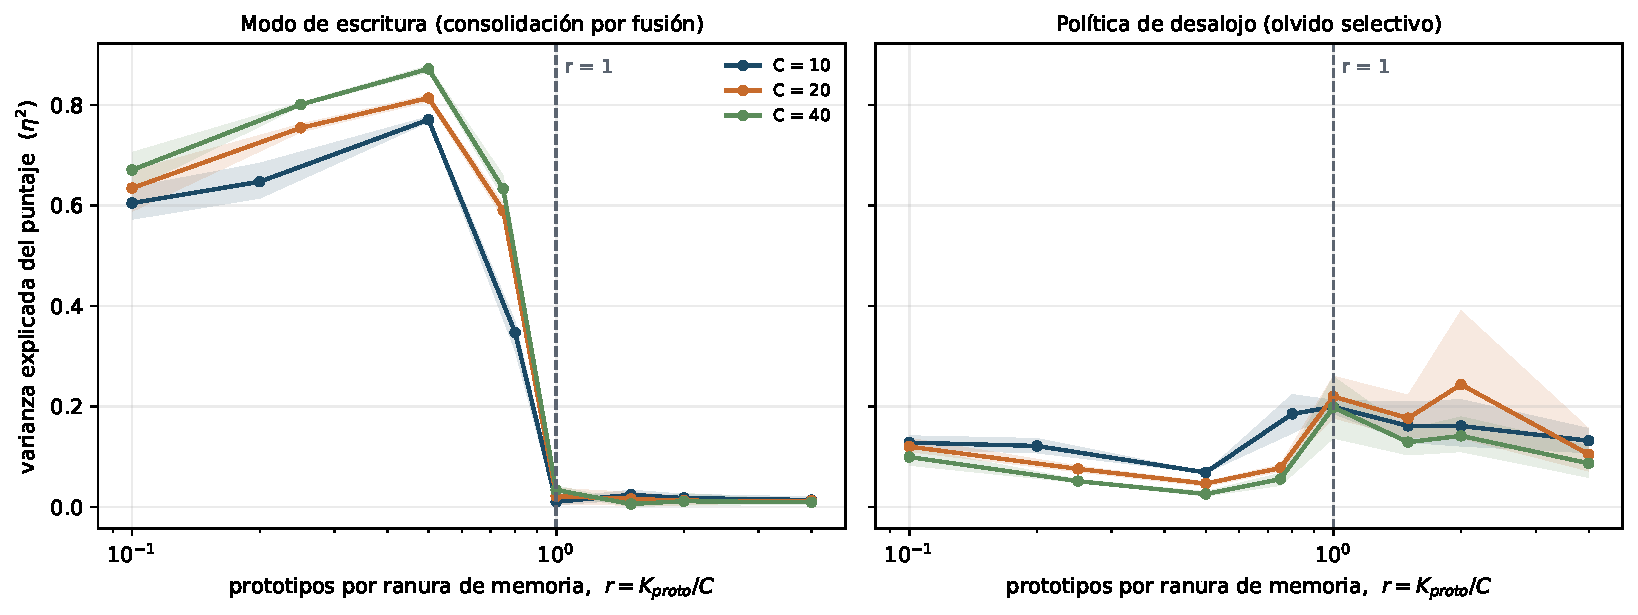
\includegraphics[width=\textwidth]{figures/fig1_threshold.pdf}
  \caption{Variance explained by write mode and by eviction policy as a function
  of the prototype-to-capacity ratio $r = K_{proto}/C$. Curves for different
  capacities collapse onto one another when plotted against $r$, which is the
  claim that the controlling variable is the ratio and not stream redundancy.
  Bands: bootstrap confidence interval over seeds.}
  \label{fig:threshold}
\end{figure*}

\subsection{The interaction between salience and eviction}
\label{sec:interaction}

The $1.4\,\%$ main effect of initial strength (Table \ref{tab:main-effects}) is
misleading read on its own. It reflects that strength modulation only
influences an architecture's behavior when a mechanism \emph{reads} that signal
---and of the four eviction policies, only \texttt{min\_strength} does.
Conditioning rare-event retention on
\texttt{\{evict: min\_strength, write: append\}}, constant strength leaves the
policy degenerate into a pseudo-random eviction
(\result{exp01_nas_full:salience_conditional.constant|pct}{3.6}\,\%), whereas
combining novelty and prediction error makes it selective
(\result{exp01_nas_full:salience_conditional.both|pct}{52.0}\,\%): a conditional
improvement of
\result{exp01_nas_full:salience_conditional_ratio|f2}{14.41}$\times$, entirely
attributable to this interaction and not to the salience gate as an isolated
mechanism.

% ═══════════════════════════════════════════════════════════════════════
\section{Comparative architecture evaluation}

Architecture search identifies the best-performing combination of axes, but it
does not evaluate the architectures as standalone memory systems. In
particular, it does not test whether each one can perform the fundamental
operation any associative memory must support: reconstructing a complete
pattern from a noisy or partial cue. This section describes a two-phase
benchmark that first admits architectures by reconstruction fidelity (R1--R4,
no capacity pressure) and then evaluates them under continuous capacity
pressure (T1--T3), over the same four architectures ---SDM, ENN (pure Hebbian
memory), Spiking-SDM (SDM with LIF-neuron activation), and a pure spiking
circuit (LIF + STDP)--- plus the e-MDB FIFO as a baseline sharing the same
design space. Table \ref{tab:benchmark} summarizes both phases.

% Generado por ember.paper_sync. No editar a mano.
\begin{table*}[t]
\centering
\caption{Two-phase evaluation. R1--R4 measure reconstruction with no capacity pressure and decide admission; T1--T3 measure retention under pressure. KiB: state held at $C=20$, $d=32$.}
\label{tab:benchmark}
\begin{tabular}{lrrrrrcrrrr}
\hline
Arch. & R1 & R2 & R3 & R4 & Mean & Gate & T1 & T2 & T3 & KiB \\
\hline
SDM & 0.672 & 0.788 & 1.000 & 0.978 & 0.859 & \checkmark & 1.000 & 0.365 & 0.875 & 131.1 \\
ENN & 0.691 & 0.938 & 1.000 & 1.000 & 0.907 & \checkmark & 0.750 & 0.344 & 0.375 & 3.1 \\
Spiking & 0.190 & 0.146 & 1.000 & 0.499 & 0.459 & $\times$ & -- & -- & -- & 105.1 \\
SpikingSDM & 0.507 & 0.433 & 0.950 & 0.588 & 0.619 & \checkmark & 0.675 & 0.158 & 0.719 & 133.0 \\
FIFO & 0.691 & 0.938 & 1.000 & 1.000 & 0.907 & \checkmark & 0.038 & 0.254 & 0.000 & 3.1 \\
\hline
\end{tabular}
\end{table*}


Every architecture except the pure spiking circuit clears the admission
threshold of 0.50
(\result{exp04_arch_benchmark:architectures.Spiking.gate.mean|f3}{0.459}\
against a gate of 0.50). ENN and FIFO get exactly the same gate score: with no
capacity pressure, ENN's merge threshold (0.85) is rarely exceeded between
near-orthogonal vectors, so every write creates a new trace and both
architectures reduce to nearest-neighbor search over the full set of stored
keys. The difference between them emerges only under capacity pressure with
structured streams, in phase 2.

The pure spiking circuit fails pattern reconstruction and noise robustness
despite forming distinguishable assemblies (perfect $A\to B$ interference). The
cause is a domain mismatch: the circuit was designed and validated on discrete
neural activation patterns; over a continuous \texttt{float32} vector,
inner-product neuron selection is sensitive to small perturbations, and a noisy
version of a stored vector activates a partially different set of neurons. This
result is not a flaw of the spiking mechanism itself ---it is the direct
motivation for EMBER's PoC-5: an integrated core combining SDM (for the
continuous-to-distributed mapping) with ENN (for the trace lifecycle).

In phase 2, SDM achieves perfect rare-event retention
(\result{exp04_arch_benchmark:architectures.SDM.battery.per_task.rare_retention}{1.000},
$\sigma=$\result{exp04_arch_benchmark:architectures.SDM.battery.per_task_std.rare_retention|f3}{0.000}
across the four seeds): rare events receive high initial strength from
prediction error, and minimum-strength eviction always displaces the routine
first. ENN, with the same strength gate and the same eviction policy, retains
less
(\result{exp04_arch_benchmark:architectures.ENN.battery.per_task.rare_retention}{0.750},
also with no seed-to-seed spread): its merge mechanism, reinforced repeatedly by
routine visits, can accumulate more strength than a rare event written only
once, though this effect is less severe than in earlier designs because the
intra-prototype spread of the current streams triggers merging less often.
Spiking-SDM retains
\result{exp04_arch_benchmark:architectures.SpikingSDM.battery.per_task.rare_retention}{0.675},
and the FIFO ---with no importance criterion at all--- is the floor among
architectures
(\result{exp04_arch_benchmark:architectures.FIFO.battery.per_task.rare_retention}{0.038},
$\sigma=$\result{exp04_arch_benchmark:architectures.FIFO.battery.per_task_std.rare_retention|f3}{0.041}:
the floor is consistent across seeds, not an artifact of a single run, though
noisier than the rest because of how close it is to zero). With a
block-differentiated prediction-error signal, the sequential-interference task
gives
\result{exp04_arch_benchmark:architectures.SDM.battery.per_task.sequential_interference|f3}{0.875}\
for SDM,
\result{exp04_arch_benchmark:architectures.ENN.battery.per_task.sequential_interference|f3}{0.375}\
for ENN, and
\result{exp04_arch_benchmark:architectures.FIFO.battery.per_task.sequential_interference|f3}{0.000}\
for the FIFO ---all three with no seed-to-seed spread. This is the comparison
that separates the three architectures by their ability to resist catastrophic
forgetting.

% ═══════════════════════════════════════════════════════════════════════
\section{Validation on real perceptual embeddings}
\label{sec:real}

All the preceding experiments run on random Gaussian vectors in
$\mathbb{R}^{32}$, which at that dimension are nearly orthogonal to one another.
This reduces cross-interference between stored patterns and could overestimate
retrieval accuracy relative to real perceptual embeddings, which exhibit
correlated structure and uneven cluster density. To answer this objection
without relying on the robot, we instrument the same grid as Section
\ref{sec:nas} on streams built from CIFAR-100 \cite{krizhevsky2009} embeddings
extracted with a pretrained ResNet-18 \cite{he2016} and reduced by PCA to the
same working dimension.

% Generado por ember.paper_sync. No editar a mano.
\begin{table*}[t]
\centering
\caption{The consolidation precondition, measured on both domains.}
\label{tab:domains}
\begin{tabular}{lrcrr}
\hline
Domain & Intra-proto. sim. & Merge reachable & $\eta^2$ write & Crossover $r$ \\
\hline
Synthetic & 0.929 & \checkmark & 1.3--81.5\,\% & 0.77 \\
CIFAR-100 & 0.401 & $\times$ & 0.0--0.4\,\% & -- \\
\hline
\end{tabular}
\end{table*}


The result, summarized in Table \ref{tab:domains}, is not that the threshold
shifts: it is that, with this extractor, the write axis is inoperative in all
five cells of the sweep. The intra-prototype cosine similarity measured on
CIFAR-100 has a median of
\result{exp05_real_embeddings:precondicion_cifar100.similitud_intra_prototipo|f3}{0.401},
well below the merge threshold
(\result{exp05_real_embeddings:precondicion_cifar100.umbral_de_fusion|f2}{0.85}),
so merging almost never triggers and $K_{effective}$ ---how many traces the
routine experience occupies after consolidation--- grows without bound with the
number of writes instead of converging to $K_{proto}$: from
\result{exp05_real_embeddings:dominios.cifar100.celdas.0.k_efectivo|int}{84}\
to \result{exp05_real_embeddings:dominios.cifar100.celdas.4.k_efectivo|int}{1435}\
traces as nominal $K$ rises from 5 to 80, with capacity fixed at 20. The
synthetic domain, in the same run, does cross normally
($r \approx \result{exp05_real_embeddings:dominios.synthetic.r_umbral|f2}{0.77}$),
confirming that the engine and the rest of the grid behave as expected.

This precondition is not a special case of rewriting the law over an effective
ratio: it is a separate binary check that comes first. One must first ask
whether the domain's intra-prototype similarity reaches the merge threshold;
only if the answer is yes does it make sense to ask how many effective
prototypes there are. On CIFAR-100 the answer to the first question is already
no, and no recomputation of $r$ ---nominal or effective--- produces a
compression regime where there is none. Silhouette-based prototype-count
estimation, moreover, becomes uninformative on this domain (confidence
intervals that reach the search ceiling in several cells), which is consistent
with the absence of compact cluster structure: this is a further reason to
treat merge reachability, measured directly by similarity, as the robust
diagnostic, rather than a derived $\hat K$.

% ═══════════════════════════════════════════════════════════════════════
\section{Validation in a real environment under partial observability}
\label{sec:minigrid}

CIFAR-100 validates the threshold law on real data, but it is still a
hand-built stream from static embeddings. A robot does not receive a stream: it
receives the consequences of its own actions, with partial observation and
temporal structure that no generator reproduces. We instrument the
\texttt{ember.envs} adapter on \texttt{MiniGrid-MemoryS13-v0} \cite{minigrid},
a navigation environment designed specifically to demand memory: the agent must
remember an object seen at the start of the episode in order to choose
correctly at the end. We compare the frontier genotype from Section
\ref{sec:nas} against the FIFO with \texttt{t1\_rare\_retention} ---the same
task that measures rarity throughout the rest of the program--- across three
conditions that change one variable at a time (Table \ref{tab:minigrid}).

% Generado por ember.paper_sync. No editar a mano.
\begin{table*}[t]
\centering
\caption{MiniGrid-MemoryS13-v0, 40 rollouts per condition. Overlap: fraction of common experiences with a prediction error equal to or greater than the least surprising rare event. Frontier / FIFO: rare-event retention.}
\label{tab:minigrid}
\begin{tabular}{llrrrr}
\hline
Policy & Surprise & Rare & Overlap & Frontier & FIFO \\
\hline
Random & Perception & 38 & 75.4\,\% & 0.0\,\% & 2.6\,\% \\
Forward-biased & Perception & 156 & 73.5\,\% & 0.0\,\% & 1.3\,\% \\
Random & Reward & 38 & 5.6\,\% & 52.6\,\% & 2.6\,\% \\
\hline
\end{tabular}
\end{table*}


\textbf{Baseline.} With a uniform random policy, both the frontier and the FIFO
sit at the rare-event retention floor. The cause is not a retrieval error
---with no capacity pressure the frontier recovers any stored trace with
similarity 1.0--- but that the one-step prediction error, computed by an online
linear transition model over the observation, does not separate the rewarded
from the merely novel: 75.4\,\% of common experiences have a prediction error
equal to or greater than the least surprising rewarded event.

\textbf{Ruling out data scarcity.} Before attributing this to a domain
precondition, the simplest explanation must be ruled out. A policy biased
toward moving forward over turning ---which does not touch the surprise
computation at all, only what gets visited--- produces $4\times$ more rewarded
episodes on the same step budget. Retention stays at the floor and the overlap
does not improve: quadrupling the data without touching the signal changes
nothing, so the problem is not a small sample.

\textbf{The signal, not the quantity.} The strength gate is motivated by the
dopaminergic account of prediction error \cite{cole2015}, but that account is
about \emph{reward}-prediction error, not perceptual. We replace the transition
model with a reward predictor ---same online linear architecture, same random
policy as the baseline, changing only what is predicted--- and the overlap
falls from 75.4\,\% to 5.6\,\%. The frontier's retention rises from
\result{exp06_minigrid:comparacion_aleatoria_prediccion.resultados.frontera.tasa|pct}{0.0}\,\%
to
\result{exp06_minigrid:comparacion_aleatoria_recompensa.resultados.frontera.tasa|pct}{52.6}\,\%
---with 38 rare events per condition, a 95\,\% Wilson interval of
[\result{exp06_minigrid:comparacion_aleatoria_recompensa.resultados.frontera.ci_low|pct}{37.3}\,\%,
\result{exp06_minigrid:comparacion_aleatoria_recompensa.resultados.frontera.ci_high|pct}{67.5}\,\%]---
while the FIFO ---which does not read the strength signal at all--- stays at
\result{exp06_minigrid:comparacion_aleatoria_recompensa.resultados.FIFO.tasa|pct}{2.6}\,\%
([\result{exp06_minigrid:comparacion_aleatoria_recompensa.resultados.FIFO.ci_low|pct}{0.5}\,\%,
\result{exp06_minigrid:comparacion_aleatoria_recompensa.resultados.FIFO.ci_high|pct}{13.5}\,\%]),
just as in the baseline. The two intervals do not overlap despite the small
sample. That only the architecture that actually consults the strength signal
improves rules out the improvement being an artifact of the predictor change:
it is specifically the salience gate working, now that it has a signal
correlated with what matters.

The salience mechanism does transfer to a real environment under partial
observability ---not automatically, but under an identifiable and correctable
precondition: surprise must be anchored in the variable that decides what
matters, and in an environment with reward that variable is reward itself, not
the perceptual novelty of the state.

% ═══════════════════════════════════════════════════════════════════════
\section{Discussion}

\subsection{The threshold law and its practical implication}

The ratio $r = K_{proto}/C$ is not an abstract quantity; for a robot it has a
direct operational interpretation. In an early, structured environment (a
warehouse, a lab), $K_{proto}$ may be small relative to the memory budget: the
robot sees the same objects and corridors repeatedly, and $r < 1$. In that
regime, merge consolidation is the most efficient strategy. Later, in a
heterogeneous or open environment, the robot encounters many distinct
situations and $r$ grows above 1; there, selective eviction by surprise and
relevance becomes the dominant requirement. The design recommendation that
follows is not to pick a regime and optimize for it: the frontier architecture
(\texttt{\{write: append, strength: both, decay: 1.0, evict: min\_strength\}})
works well in both regimes because it never depends on merging ---which fails
above $r=1$--- and always exploits the importance signal, which is
regime-neutral by construction.

\subsection{The spiking circuit and the motivation for PoC-5}

That the pure spiking circuit does not pass the reconstruction gate is a result
of the design space, not a deficiency of the spiking mechanism itself. PoC-3
established that LIF+STDP circuits form reliable engrams and support pattern
completion in their native domain. The gap this work identifies is that the
bridge between continuous input vectors and discrete neural assemblies does not
yet exist. That bridge is precisely the goal of EMBER's PoC-5: an integrated
core combining SDM ---for the continuous-to-distributed mapping--- with ENN
---for the trace lifecycle--- as a single \emph{Cognitive Node} with a complete
engram lifecycle.

\subsection{The FIFO is the right contrast}

Mapping the e-MDB FIFO to the genotype \texttt{\{read: nn, write: append,
strength: constant, decay: 1.0, evict: fifo, reinforce: 0.0\}} is deliberately
generous: the real \texttt{EpisodicBuffer} has no content-addressable retrieval
at all. Even with that advantage, it lands in the bottom quartile of the
genotype space and is the floor among architectures evaluated in the two-phase
benchmark. This is not a criticism of the e-MDB architecture, which was
designed with a different primary goal (motivational systems and policy
learning, not memory); it is a precise claim that the episodic buffer, as
implemented today, is inadequate for the LOLA operating regime, and it
motivates integrating EMBER as a direct improvement with a quantified gap to
close.

\subsection{The precondition as a deployable diagnostic}

The finding of Section \ref{sec:real} gives the robot something more useful than
a generalization warning: a check it can run online without knowing anything
about the environment. Intra-prototype similarity is measured directly on the
vectors the memory is already receiving, and comparing it against the merge
threshold decides ---before the write axis matters at all--- whether it is
worth the memory attempting to consolidate in the first place. A robot that
monitors this quantity can tell, with no external instrumentation, whether it
is in a regime where merging helps or where it is simply wasted work.

\subsection{The source of surprise matters as much as its existence}

Section \ref{sec:minigrid} generalizes this lesson beyond merging. The
synthetic and CIFAR-100 designs share a silent assumption: that the surprise
signal feeding the strength gate already comes aligned with what the robot
needs to remember. That assumption is free when the generator sets it by hand;
in a real environment one must choose \emph{what to predict}, and that choice
determines whether the mechanism has anything to protect. Predicting the
observation produces a signal that reacts to anything perceptually new,
rewarded or not. Predicting the reward produces a signal that reacts
specifically to what the robot has reason to remember. The frontier
architecture is the same in both cases ---the genotype does not change--- but
it only works when the signal it receives is the right one. The salience gate
is not a mechanism that works or fails in the abstract: it is a mechanism that
inherits the quality of its input, and choosing that input is a design decision
as consequential as any axis of the search space.

% ═══════════════════════════════════════════════════════════════════════
\section{Limitations and future work}

The real-data validation of Section \ref{sec:real} uses a single extractor
(ResNet-18 pretrained on ImageNet, PCA to 32 dimensions) on a single dataset
(CIFAR-100) and a single capacity ($C=20$). We do not know whether the
intra-class similarity of 0.401 is a property of the visual domain, of the
extractor, or of the combination of both: an extractor fine-tuned on the target
domain, or the merge threshold (fixed at 0.85 from the synthetic design)
recalibrated per domain, could give a different result. Neither reading is
ruled out by this experiment; distinguishing them is future work.

Silhouette-coefficient prototype-count estimation, which works tightly on
synthetic streams, produces uninformative confidence intervals on CIFAR-100
(reaching the search ceiling in several cells). This is consistent with the
absence of compact cluster structure in that domain, but it means any claim
about the real $\hat K_{proto}$ must be reported with its interval, never as a
point integer.

The MiniGrid validation of Section \ref{sec:minigrid} uses a single environment
(\texttt{MemoryS13}) and a single exploration policy besides the forward-biased
one; extending to POPGym and to trained policies is left as future work.

% ═══════════════════════════════════════════════════════════════════════
\section{Conclusion}

We present EMBER, a research program on bioinspired episodic memory for
cognitive robots, with four empirical contributions. Exhaustive architecture
search reveals that the relative importance of bioinspired memory mechanisms is
not fixed: it depends on the operating regime, characterized by the ratio
between recurring experience prototypes and memory capacity. Below a threshold
near 1, merge consolidation dominates; above it, selective eviction by strength
dominates. Critically, the salience mechanism at encoding ---the one the
bioinspired-memory literature most motivates--- shows a negligible main effect
yet becomes the decisive differentiator in the selection regime when combined
with minimum-strength eviction, recovering fourteen times the rare-event
retention of an architecture without that gate. The architecture benchmark
confirms these findings: SDM with a prediction-error gate is the only evaluated
architecture that simultaneously achieves high reconstruction fidelity and
perfect rare-event retention, while the e-MDB FIFO sits at the floor in every
condition. The pure spiking circuit, though validated in its native domain,
does not yet transfer to continuous input vectors, identifying PoC-5 ---EMBER's
integrated core--- as the next critical implementation milestone. Instrumenting
the same law on real perceptual embeddings exposes a precondition that no
synthetic design reveals on its own: without sufficient intra-prototype
similarity, there is no prototype-to-capacity ratio, nominal or effective, that
produces a compression regime. Far from weakening the threshold law, this
precondition turns it into an online-measurable quantity that a robot can use
to decide, with no prior knowledge of its environment, whether consolidation is
worthwhile. Finally, validating the salience mechanism in a real environment
under partial observability reveals an analogous precondition and, unlike the
previous one, resolves it: rare-event retention stays at the floor with a
perceptual surprise signal, we rule out data scarcity, and it rises to more
than half when the signal is anchored in reward rather than in state novelty
---without changing either the genotype or the exploration policy. The salience
mechanism works in a real domain; what it needs is to be fed the right signal.

\section*{Code and data availability}

The design space, the evaluation tasks, the six experiments and the measured
results (\texttt{results/**/*.json}, versioned alongside the code) backing every
table, figure and number in this paper will be released under an open license
after the review process, to preserve the anonymity of the double-blind
process.

\bibliographystyle{IEEEtran}
\bibliography{refs}

\end{document}
